\documentclass[11pt]{article}
\usepackage{geometry} % Pour passer au format A4
\geometry{hmargin=1cm, vmargin=1cm} % 

% Page et encodage
\usepackage[T1]{fontenc} % Use 8-bit encoding that has 256 glyphs
\usepackage[english,french]{babel} % Français et anglais
\usepackage[utf8]{inputenc} 

\usepackage{lmodern}
\setlength\parindent{0pt}

% Graphiques
\usepackage{graphicx,float,grffile}

% Maths et divers
\usepackage{amsmath,amsfonts,amssymb,amsthm,verbatim}
\usepackage{multicol,enumitem,url,eurosym,gensymb}

% Sections
\usepackage{sectsty} % Allows customizing section commands
\allsectionsfont{\centering \normalfont\scshape}

% Tête et pied de page

\usepackage{fancyhdr} 
\pagestyle{fancyplain} 

\fancyhead{} % No page header
\fancyfoot{}

\renewcommand{\headrulewidth}{0pt} % Remove header underlines
\renewcommand{\footrulewidth}{0pt} % Remove footer underlines

\newcommand{\horrule}[1]{\rule{\linewidth}{#1}} % Create horizontal rule command with 1 argument of height

%----------------------------------------------------------------------------------------
%	Début du document
%----------------------------------------------------------------------------------------

\begin{document}

%----------------------------------------------------------------------------------------
% RE-DEFINITION
%----------------------------------------------------------------------------------------
% MATHS
%-----------

\newtheorem{Definition}{Définition}
\newtheorem{Theorem}{Théorème}
\newtheorem{Proposition}{Propriété}

% MATHS
%-----------
\renewcommand{\labelitemi}{$\bullet$}
\renewcommand{\labelitemii}{$\circ$}
%----------------------------------------------------------------------------------------
%	Titre
%----------------------------------------------------------------------------------------

\setlength{\columnseprule}{0pt}

\section*{Evaluation CERCLES}

\horrule{2px} 

\subsection*{Restituer}
\textbf{Donner la définition précise d'un cercle}\\
\begin{minipage}{\linewidth}
\vspace{18pt}
. \dotfill \vspace{12pt} \\
. \dotfill \vspace{12pt} \\
. \dotfill \vspace{12pt} \\
. \dotfill \vspace{12pt} \\
. \dotfill \vspace{12pt} \\
\end{minipage}

\textbf{\textit{Les exercices 1, 2 et 3 sont à faire au dos de la copie.}}

\subsubsection*{EX1}
	\begin{itemize}
	\item Placer 10 points à une distance 4.6cm du point A.
	\end{itemize}


\subsubsection*{EX2}
	\begin{itemize}
	\item Tracer un carré ABCD de côté 5cm.
	\item Soit I le point d'intersection de ses diagonales.
	\item Tracer un cercle de centre I et de rayon 3cm.
	\item Tracer un cercle de centre B et de rayon 5cm.
	\end{itemize}



\subsection*{EX3 - Reproduire}
	\begin{figure}[H]
		\centering
		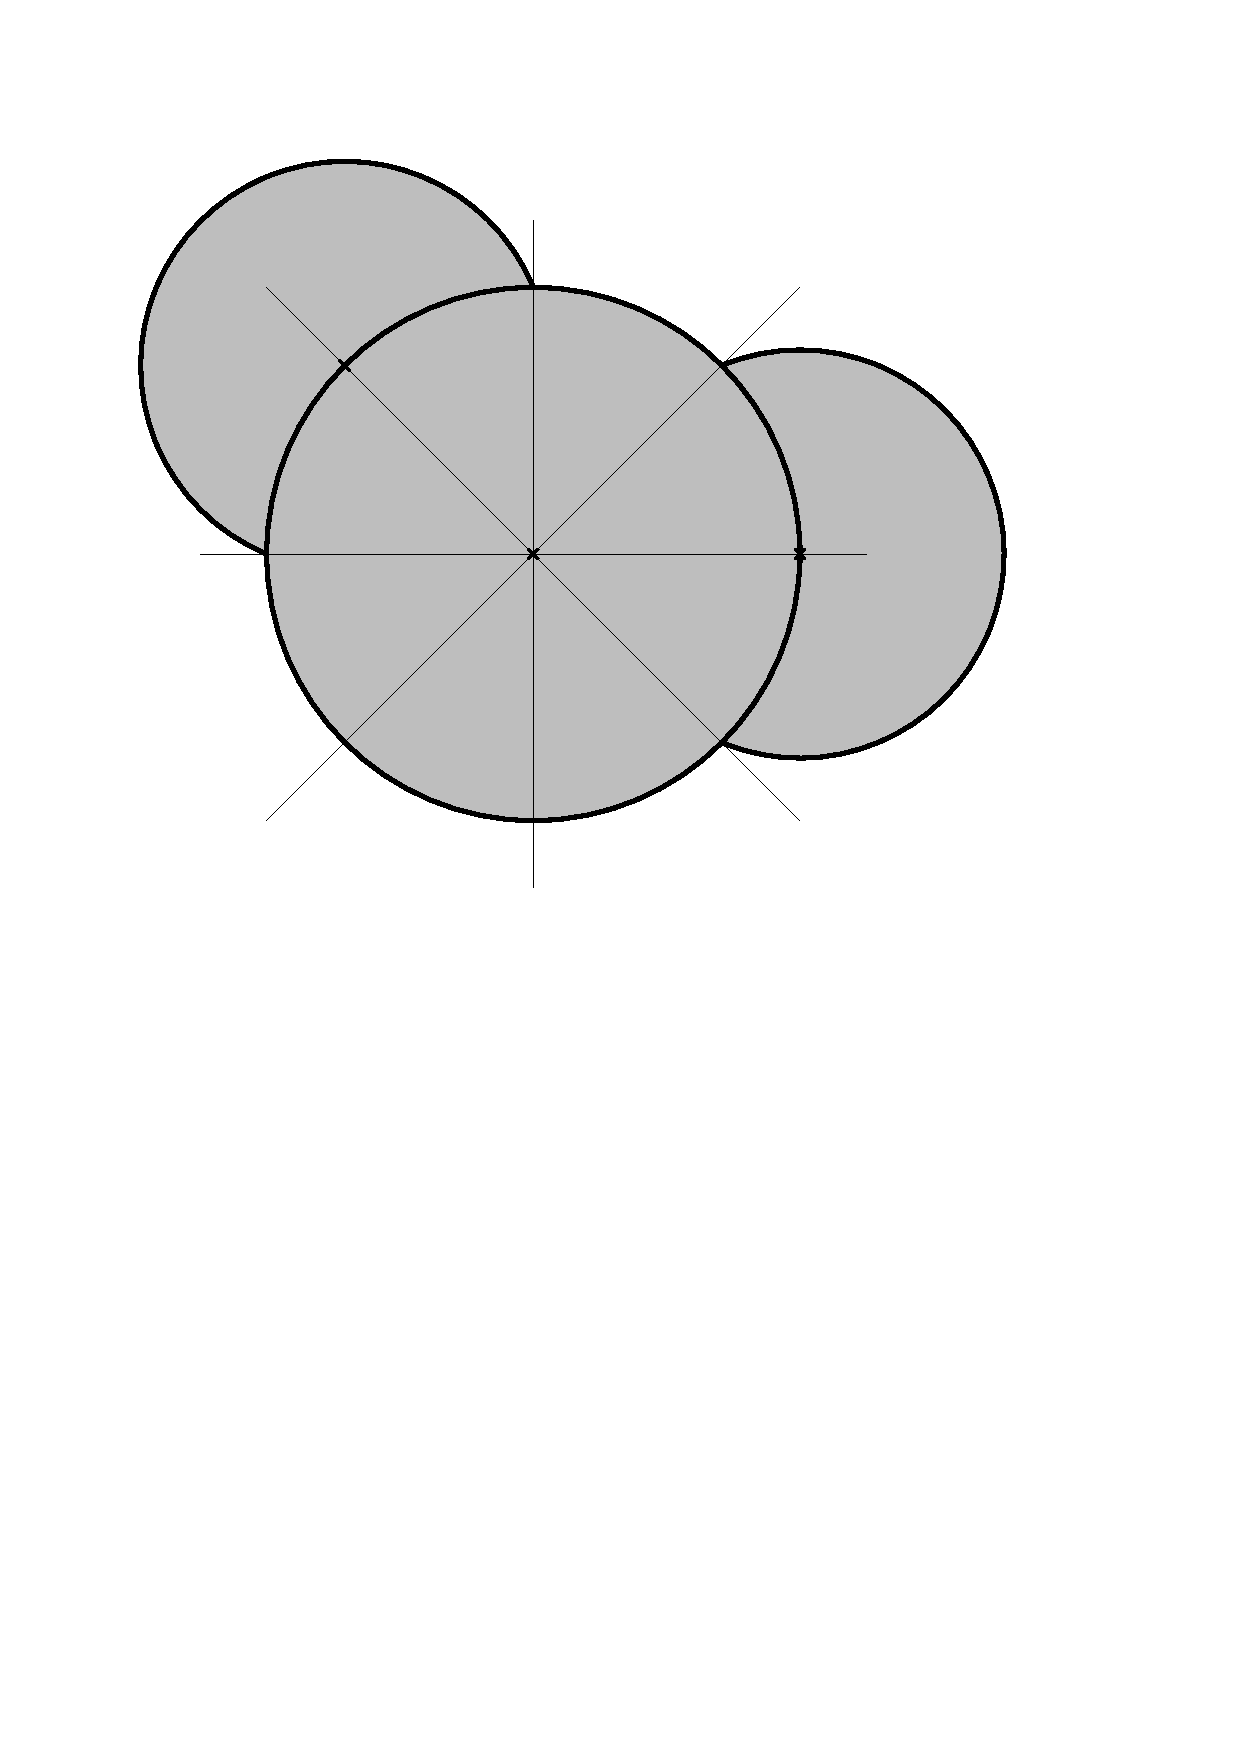
\includegraphics[width=0.6\linewidth]{6x6-cercles/sources/mol1.pdf}
	\end{figure}


\newpage

\subsection*{EX1 \hspace{10cm} EX2} 


\vspace{12cm}

\subsection*{EX3}
	\begin{figure}[H]
		\centering
		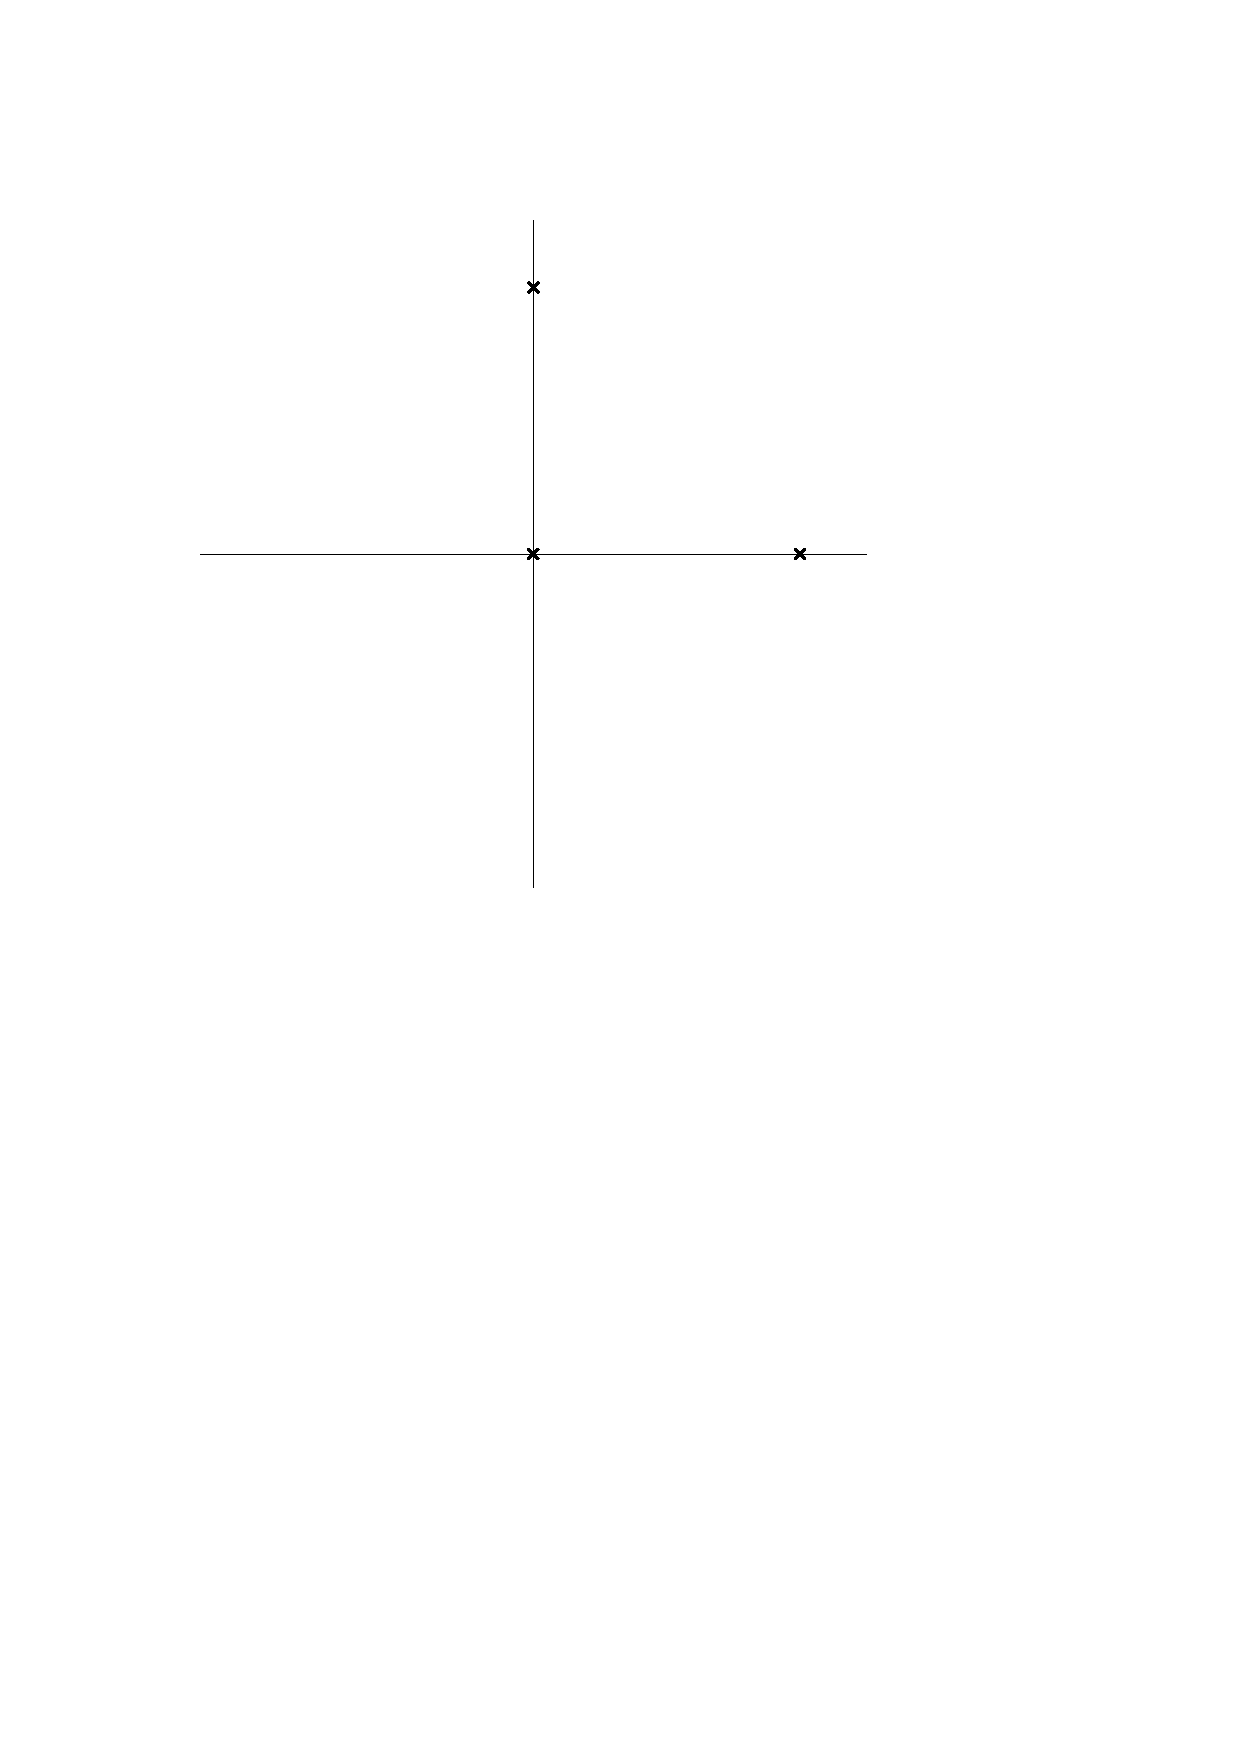
\includegraphics[width=0.6\linewidth]{6x6-cercles/sources/mol2.pdf}
	\end{figure}



\end{document}